%%=============================================================================
%% Funcionele Analyse
%%=============================================================================

\chapter{Functionele Analyse}
\label{ch:funcioneleanalyse}


\section{Situatie as is}
\begin{figure}[h]
\centering
\begin{minipage}[t]{0.49\textwidth}   
    \includegraphics*[width=1\textwidth]{img/d365productionControl1}
    \caption{D365FO dashboard}
\end{minipage}
\begin{minipage}[t]{0.49\textwidth}
    \includegraphics*[width=1\textwidth]{img/d365productionControl2}
    \caption{Overzicht alle modules binnen D365FO}
\end{minipage}
\end{figure}
    
Dit onderzoek zal zich toespitsen op de Job Card Device module binnen D365FO. Op bovenstaande figuren ziet men screenshots uit het D365FO dasboard. Eens ingelogd ziet een gebruiker deze schermen, aangepast voor hem. Zo zal een productiemedewerker bijvoorbeeld aanzienlijk minder informatie beschikbaar hebben. De module Personnel Management is voor hem bijvoorbeeld niet van toepassing en bijgevolg zal de productiemedewerker deze niet zien. Dit geldt ook voor andere irrelevante modules. 

Eens de gebruiker heeft genavigeerd naar de Production Control module zal hij kunnen kiezen voor de job card Device module. Deze module zal, gelijkaardig aan de chatbot, eerst vragen om in te loggen met zijn badgeID (zie onderstaand). Dit omdat het niet mogelijk (mag zijn) is om acties uit te voeren binnen de job card Device zonder ingelogd te zijn. 

\begin{figure}[H]
    \centering
    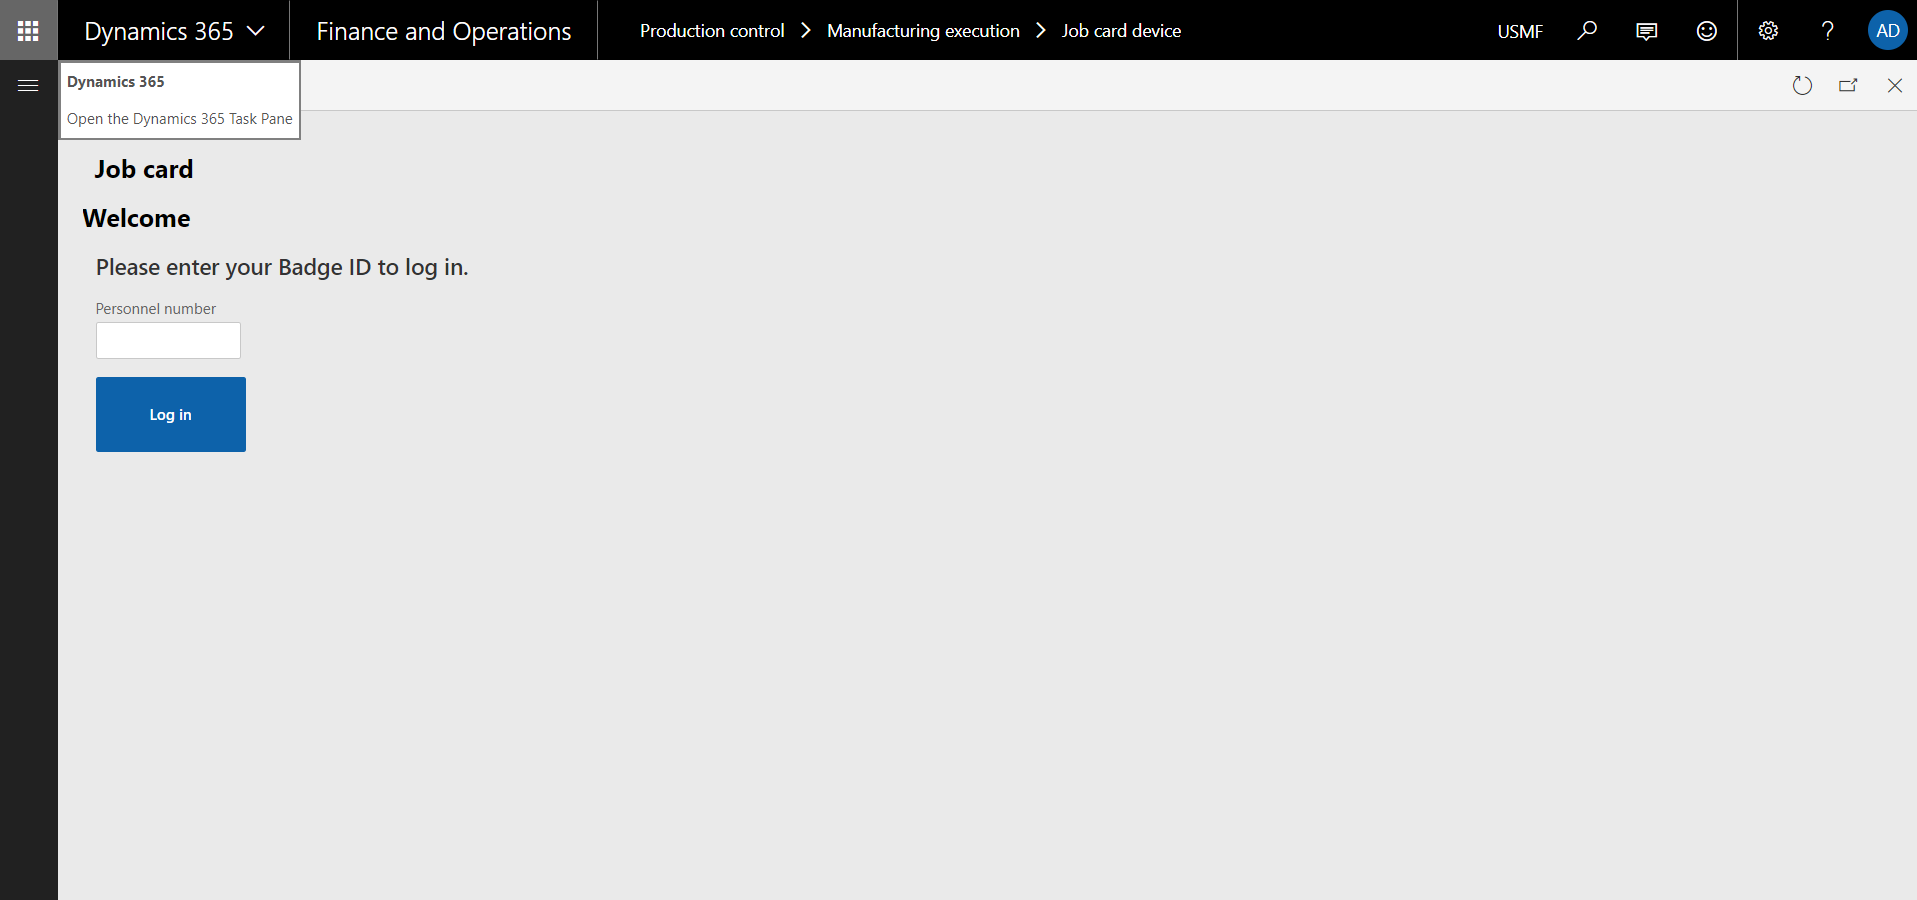
\includegraphics[width=0.8\textwidth]{img/d365productionControl3.png}
    \caption{Login-scherm Job Card Device module}
\end{figure}

Eens ingelogd komt de gebruiker dan in de Job Card Device module terecht (zie onderstaande figuur). Dit is de effectieve module waar dit onderzoek zich op zal toespitsen. De opzet is niet om de volledige module te dupliceren d.m.v. een bot, maar slechts enkele delen. Het is immers voldoende om die specifieke delen te behandelen, om aan te kunnen tonen dat een chatbot gemaakt in het MS Bot Framework in staat is om CRUD-operaties uit te voeren in D365FO. 
\begin{figure}[h]
    \centering
    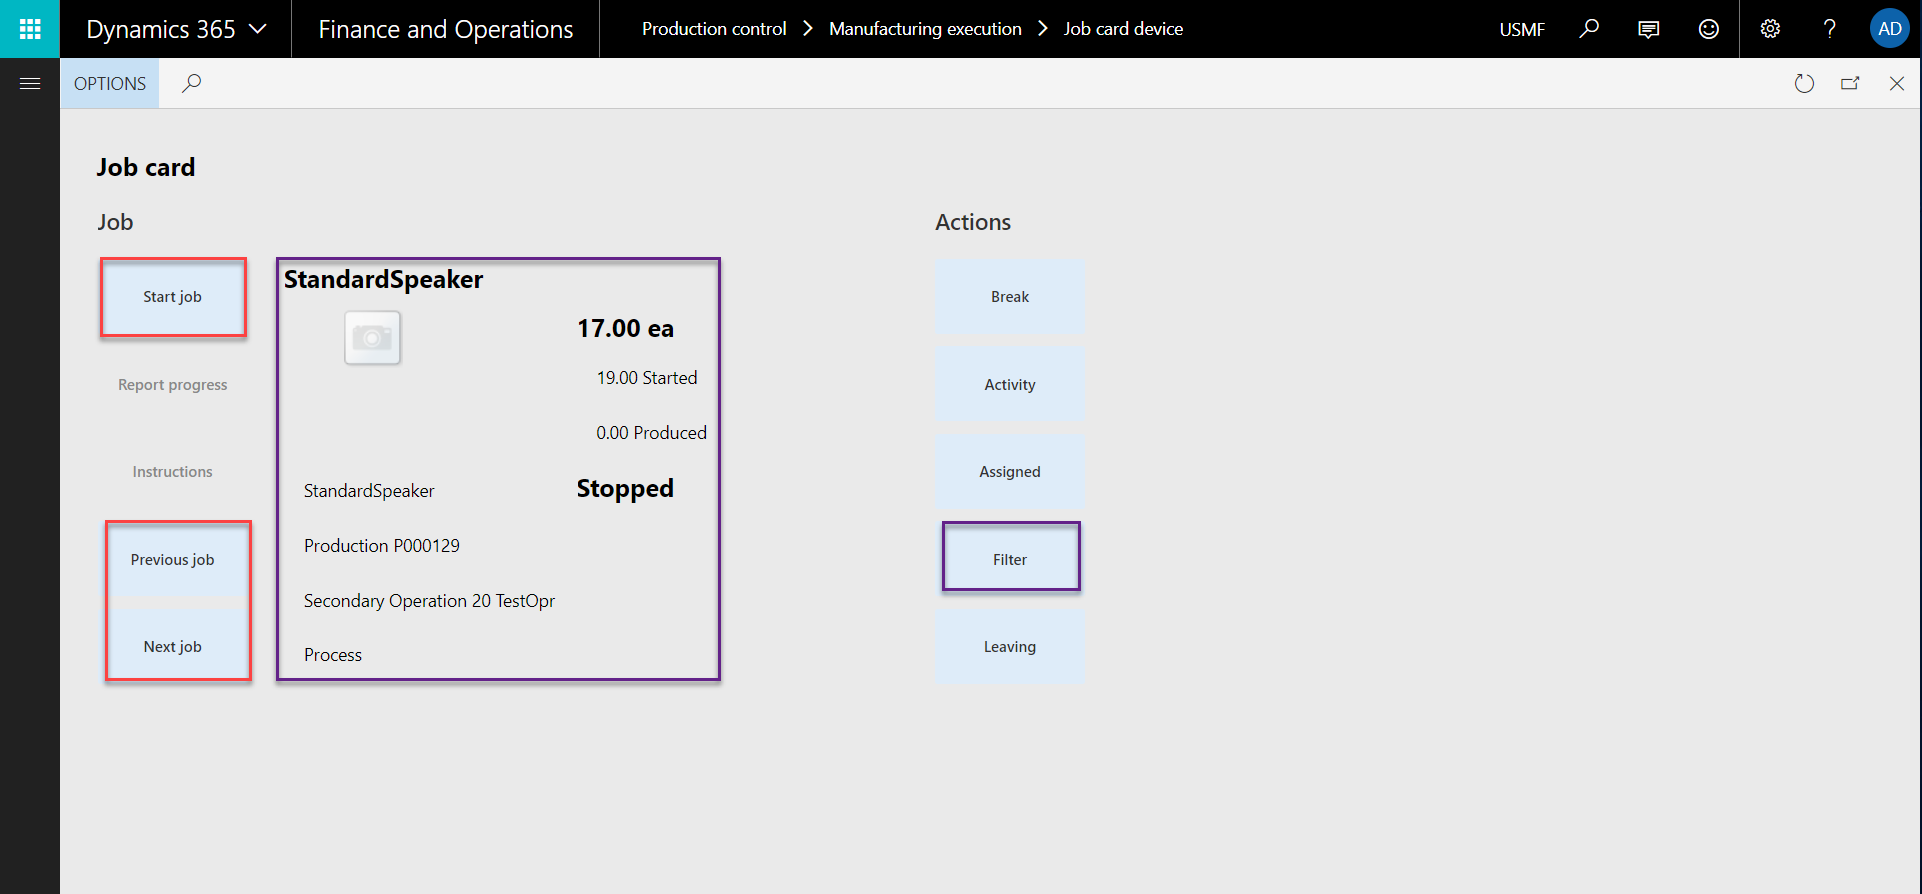
\includegraphics[width=0.8\textwidth]{img/d365productionControl4.png}
    \caption{Job Card Device module}
\end{figure}
Indeling scherm: De linkerzijde (zie rode kaders) omvat functionaliteiten die van toepassing zijn op een productie order. De knoppen aangeduid met een kader zullen in de chatbot verwerkt worden. Zo zal het dus mogelijk zijn om een job te starten (of stoppen, indien van toepassing), en om te navigeren tussen verschillende productie orders. De paarse kaders zullen ook verwerkt worden, namelijk in die zin dat het ook mogelijk zal zijn om informatie te zien over een productie order. Aanvullend zal er in de chatbot ook per productie order een bill of materials getoond worden. Dit was een extra requirement van de opdrachtgever (delaware), want een BOM is immers zeer relevante informatie voor een productiemedewerker. 


\section{Proof of concept}
Bij het onderzoek werd eerst een functionele analyse gemaakt op maat van het beoogde proof of concept. Allereerst werd hiervoor een user story opgemaakt om de scope van het onderzoek te bepalen. In onderstaande afbeelding ziet men een visuele representatie van het BPMN diagram. Voor een afbeelding op ware grootte kunnen de bijlagen geraadpleegd worden. 

\begin{figure}[h]
    \centering
    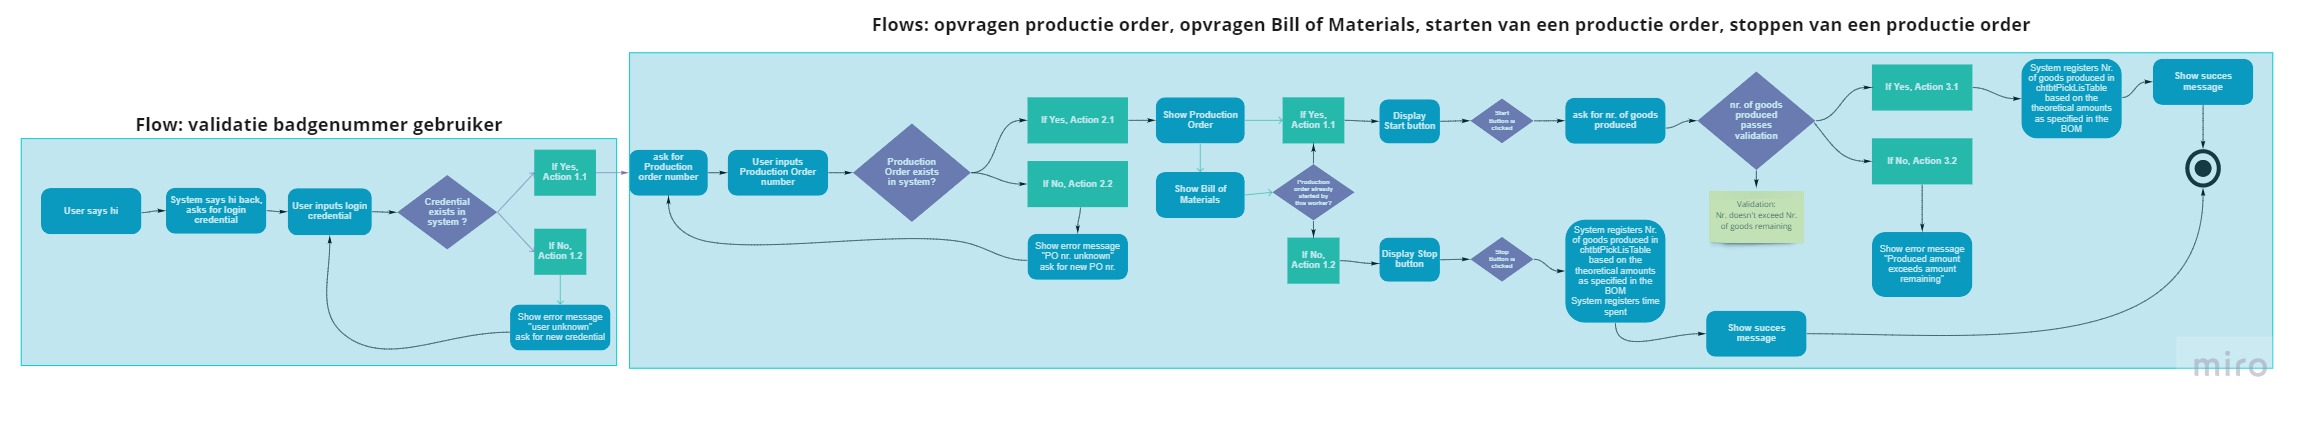
\includegraphics[width=1\textwidth]{img/HappyFlows.jpg}
    \caption{Business Process Model and Notation diagram POC }
\end{figure}

Enkele belangrijke opmerkingen: 
Het linkerdeel van het BPM? omvat must-have 5 (zie functionele requirements hieronder). Van zodra deze stap voldaan is kan de gebruiker acties uitvoeren in de chatbot, en niet eerder. Deze stap zal dus recurrent voorkomen bij alle functionaliteiten van de bot.

Verder zullen er er ook nog andere functionaliteiten in zitten die niet in het BPMN gedefinieerd zijn. Voorbeelden hiervan zijn nice to haves 3 en 4. Aangezien de flows voor deze functionaliteiten uit zéér weinig stappen bestaan, en dus in enige mate triviaal zijn. Daarom werd het opstellen van flows voor deze stappen als buiten de scope van dit onderzoek beschouwd. 

\subsubsection{functionele requirements}

Must haves:
\begin{enumerate}
    \item Er wordt een proof-of-concept gebouwd in het Microsoft Bot Framework. 
    \item Bovengenoemde bot gebruikt LUIS voor het interpreteren van natuurlijke zinnen naar commando's. 
    \item Ook moet de bot gepaste CRUD operaties kunnen uitvoeren in D365FO.
    \item Aan de hand van de MS Bot Connector Service moet de bot ook gehost kunnen worden op Azure en op Webchat. 
    \item De gebruiker kan inloggen adhv een badgeID (zonder deze badgeID kan de gebruiker niks doen. Validatie: badgeID bestaat in D365FO.)
    \item Eens ingelogd kan de gebruiker een aantal acties beginnen die voor hem van toepassing zijn:  
    \subitem De gebruiker kan een productieorder bekijken (titel, hoeveelheid en productieordernummer).
    \subitem De gebruiker kan de bill of materials zien van een productieorder (verschillende onderdelen, hoeveelheid en hoeveelheid per series)
    \subitem De gebruiker kan een productieorder starten. Hiervoor moet hij eerst een hoeveelheid invullen (validatie: hoeveelheid is kleiner of gelijk aan de resterende hoeveelheid)
    \subitem De gebruiker kan een productieorder stoppen (validatie: dit is enkel mogelijk als de gebruiker deze actie heeft gestart.) 
    
\end{enumerate}

Nice to haves:
\begin{enumerate}
    \item De gebruiker kan aan de hand van spraakherkenning communiceren met de bot.
    \item De gebruiker kan aan de hand van stemherkenning herkend worden door de bot, waardoor inloggen met badgeID niet langer noodzakelijk is
    \item De gebruiker kan aan de hand van een help-menu bekijken wat zijn opties zijn (welke stappen hij kan uitvoeren d.m.v. de bot)
    \item De gebruiker kan een overzicht zien van alle presentatie-mogelijkheden binnen de bot. Deze nice to have is louter voor presentatie doeleinden bestemd. Zo moet het mogelijk kunnen zijn om te raadplegen welke soorten informatie, en in welke vorm, allemaal raadpleegbaar zijn binnen de bot (foto's, video's, hyperlinks, etc.)
\end{enumerate}

Enkele belangrijke opmerkingen:
De focus voor dit onderzoek ligt niet op het coderen van zo veel mogelijk functionaliteiten, aangezien dit na de eerste keer veel repetitief werk met zich meebrengt. Het werd daarom als voldoende beschouwd door de opdrachtgever (delaware) wanneer er duidelijk vastgesteld kon worden dat er communicatie tussen D365FO en de bot mogelijk is (zie must have 3). Later in dit onderzoek zal samengevat worden wat de aangeraden stappen en best-practices hiervoor zijn.  Er zal daarom meer toegespitst worden op de werkwijze, en onder andere de voor- en nadelen. 

Tenslotte kunnen bovenstaande functionele requirements samenvattend weergegeven worden in volgende user stories: 

\begin{figure}[h]
    \centering
    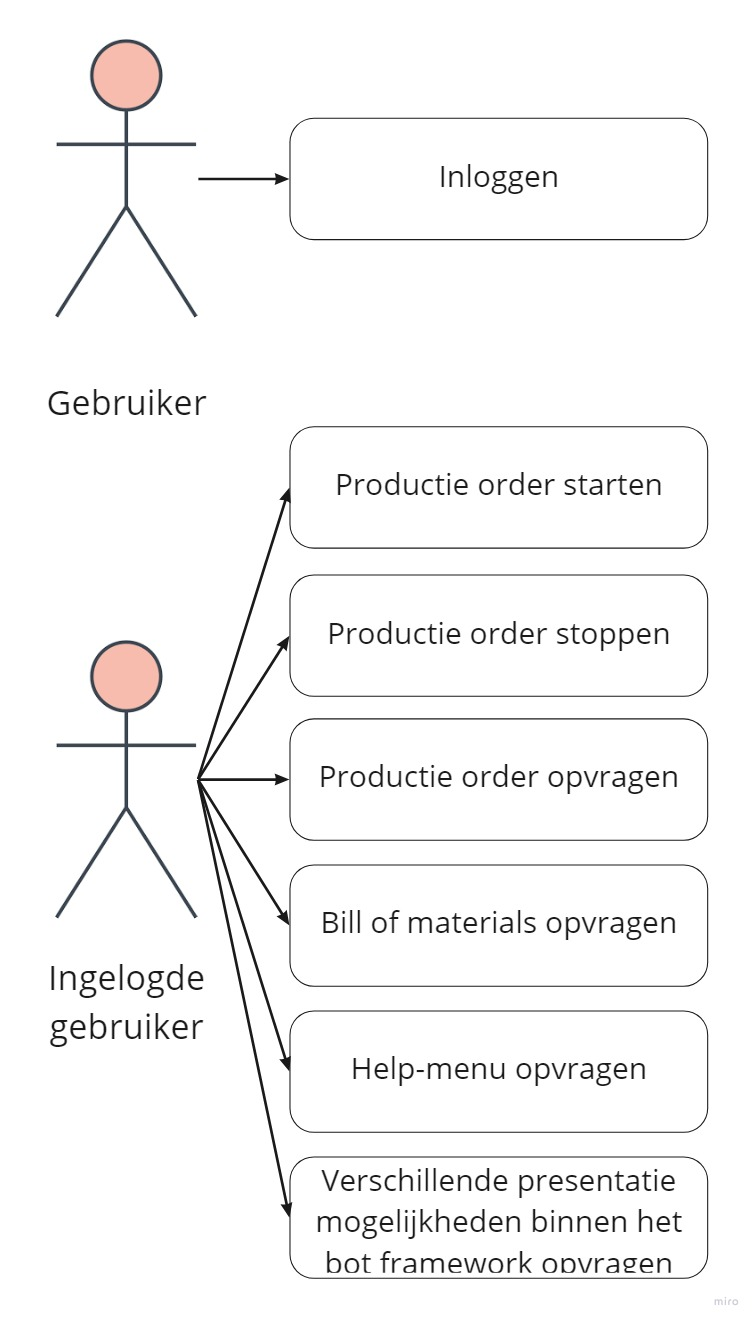
\includegraphics[width=0.32\textwidth]{img/UserStories.jpg}
    \caption{User stories POC }
\end{figure}


 
